\documentclass[11pt]{article}
\usepackage[margin=1in]{geometry}
\usepackage{amsmath,amssymb,booktabs,graphicx,microtype}
\usepackage[hidelinks]{hyperref}
\newcommand{\E}{\mathbb E}

\title{Long-chain Gallavotti--Cohen diagnostic\\
for the boundary-driven resonant NLS model}
\author{}
\date{29 August 2026}

\begin{document}
\maketitle

\section*{Question and admissible conclusion}

For the driven Cartesian NLS chain at $(T_L,T_R)=(10,2)$ and
$n=10,20,30,40$, we test the long-time scaled cumulant-generating-function
(SCGF) symmetry
\begin{equation}
  \psi_n(k)=\psi_n(1-k),\qquad
  \psi_n(k)=\lim_{t\to\infty}\frac1t
  \log\E_{\rm NESS}\!\left[e^{-k\Sigma_R(t)}\right].
  \label{eq:gc}
\end{equation}
The simulation can establish numerical consistency only for the resolved tilt
pairs, finite horizons, clone populations, timesteps, and chain lengths.  It
does not prove the analytic theorem for all $k$, all $n$, or the infinite-chain
limit.

\section{Thermodynamic observable and normalization}

Heat $Q_r$ is positive when bath $r$ transfers energy into the system.  The
Cartesian code advances the physical energy $E=H/2$, so its equilibrium law
$e^{-E/T}=e^{-H/(2T)}$ is exactly the manuscript convention.  The medium
entropy is
\begin{equation}
  \Sigma_{\rm m}=-\frac{Q_L}{T_L}-\frac{Q_R}{T_R}.
\end{equation}
Using the measured first law $Q_L+Q_R=\Delta E+r_{\rm FL}$ gives the
right-boundary gauge
\begin{equation}
  \Sigma_R=-\left(\frac1{T_R}-\frac1{T_L}\right)Q_R=-0.4Q_R,
  \qquad
  \Sigma_R-\Sigma_{\rm m}=\frac{\Delta E}{T_L}+O(r_{\rm FL}).
  \label{eq:gauge}
\end{equation}
Thus $\Sigma_R$ and $\Sigma_{\rm m}$ have the same long-time SCGF when the
required endpoint-energy exponential moments exist.  Their finite-time
difference is measured rather than assumed to vanish.

\section{Estimator and frozen acceptance gates}

The dynamics is simulated in projection-free Cartesian variables with a
Hamiltonian implicit-midpoint substep and exact discrete bath-heat increments.
Burn-in is $B=500$ and the production timestep is $\Delta t=5\times10^{-4}$.
The rare-event estimator uses a controlled Gaussian proposal followed by
fixed-population cloning.  For every bath step the exact original/proposal
transition-density ratio is included in the weight.  Consequently the control
changes sampling efficiency but not the target finite-step Feynman--Kac
expectation.

The proposal scale $0.5$ and selection interval $2$ were frozen using only
weight-ESS, ancestry, and direct-calibration diagnostics.  The GC residual was
not used to choose them.  Four independent seeds are required for every
reported member.  Acceptance additionally requires zero midpoint failures,
minimum per-selection weight ESS $\ge0.1N_c$, a paired 95\% interval containing
zero, absolute paired and late-half residuals no larger than $0.01$, and
agreement under observation-time and clone-population increases.  Timestep
halving and a changed selection interval are tested independently.

The strongest predeclared pair $(0.3,0.7)$ is resolved at $n=10$.  Its
high-tilt member loses support for $n\ge20$, so those failures are retained and
the already predeclared secondary pair $(0.4,0.6)$ is used for
$n=20,30,40$.

\section{Independent validation controls}

The following controls do not use the observed GC residual as a tuning target.
\begin{itemize}
  \item Zero-control change-of-measure and Gaussian-model cloning self-tests
  pass, as do address and undefined-behavior sanitizer tests.
  \item Arbitrary-chain forward/reverse one-step path-ratio controls pass for
  $n=10,20,40$.  The initial $n=30$ sample narrowly failed its forward IFT
  interval; an independently seeded $N=5\times10^5$ replication passes both
  IFT directions and gives Crooks slope $0.9941$.
  \item The direct million-block data satisfy the gauge identity in
  \eqref{eq:gauge}; its RMS discrepancy is between $6.1\times10^{-6}$ and
  $1.9\times10^{-5}$ across the four chain lengths.
  \item Where both direct exponential averages have support, the controlled
  $t=20$ SCGF agrees with direct sampling within uncertainty.  At low tilt the
  directly sampled right-gauge/medium-entropy SCGF difference decreases with
  time, as expected for the endpoint term in \eqref{eq:gauge}.
\end{itemize}

\begin{figure}[ht]
  \centering
  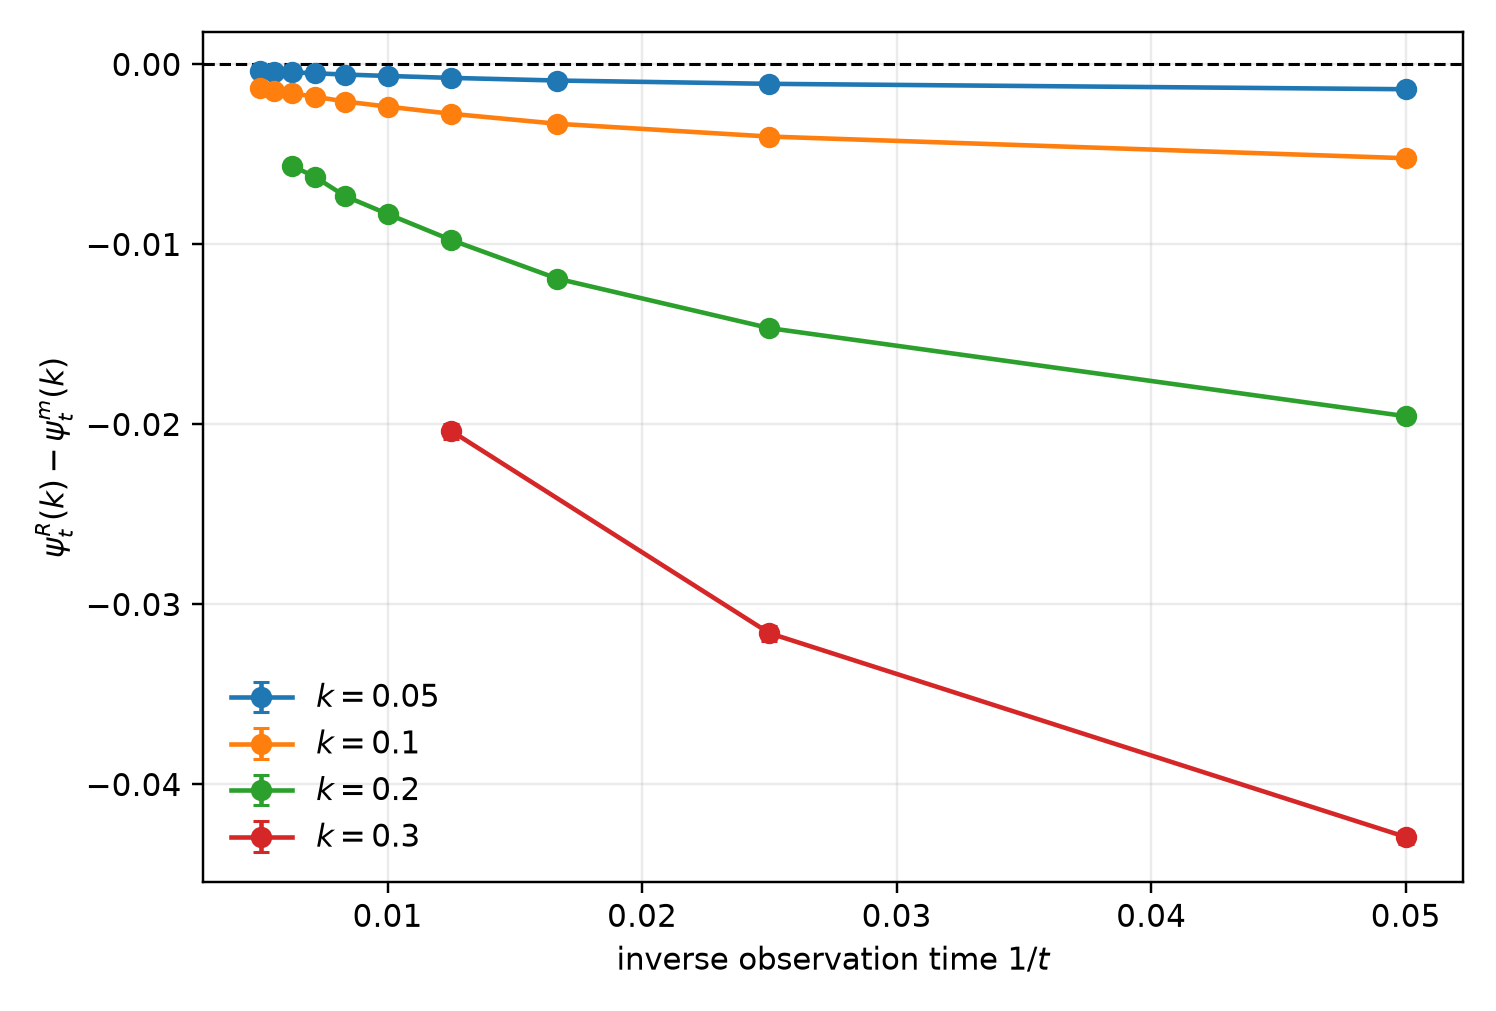
\includegraphics[width=0.78\textwidth]{../gauge_convergence_analysis/gauge_convergence_n40.png}
  \caption{Finite-time endpoint-gauge diagnostic at $n=40$.  Equality is not
  imposed at finite time; the measured difference decreases with horizon in
  the low-tilt support region.}
  \label{fig:gauge}
\end{figure}

\clearpage
\section{Long-chain SCGF results}

Table~\ref{tab:gc} contains only the rows frozen in
\texttt{FINAL\_RESULT\_SPEC.csv}.  The confidence intervals use the variation
among four independent runs rather than clone-to-clone variation.

\begin{table}[ht]
\centering
\small
\caption{Resolved GC pairs at their pre-specified final horizons.  Here
$D=\psi_t(k)-\psi_t(1-k)$.}
\label{tab:gc}
\begin{tabular}{rrrrrrrll}
\toprule
$n$ & pair & $N_c$ & $t$ & $\psi_t(k)$ & $\psi_t(1-k)$ & $D$ & 95\% CI for $D$ & core audit \\
\midrule
10 & $(0.3,0.7)$ & 2048 & 60 & -0.17878 & -0.17870 & -0.00008 & $[-0.00995,+0.00980]$ & pass \\
20 & $(0.4,0.6)$ & 1024 & 60 & -0.08576 & -0.08237 & -0.00339 & $[-0.01208,+0.00530]$ & pass \\
30 & $(0.4,0.6)$ & 2048 & 60 & -0.04855 & -0.04498 & -0.00357 & $[-0.00824,+0.00109]$ & unresolved \\
40 & $(0.4,0.6)$ & 1024 & 120 & -0.03259 & -0.03709 & +0.00450 & $[-0.00234,+0.01134]$ & pass \\
\bottomrule

\end{tabular}
\end{table}

\begin{figure}[ht]
  \centering
  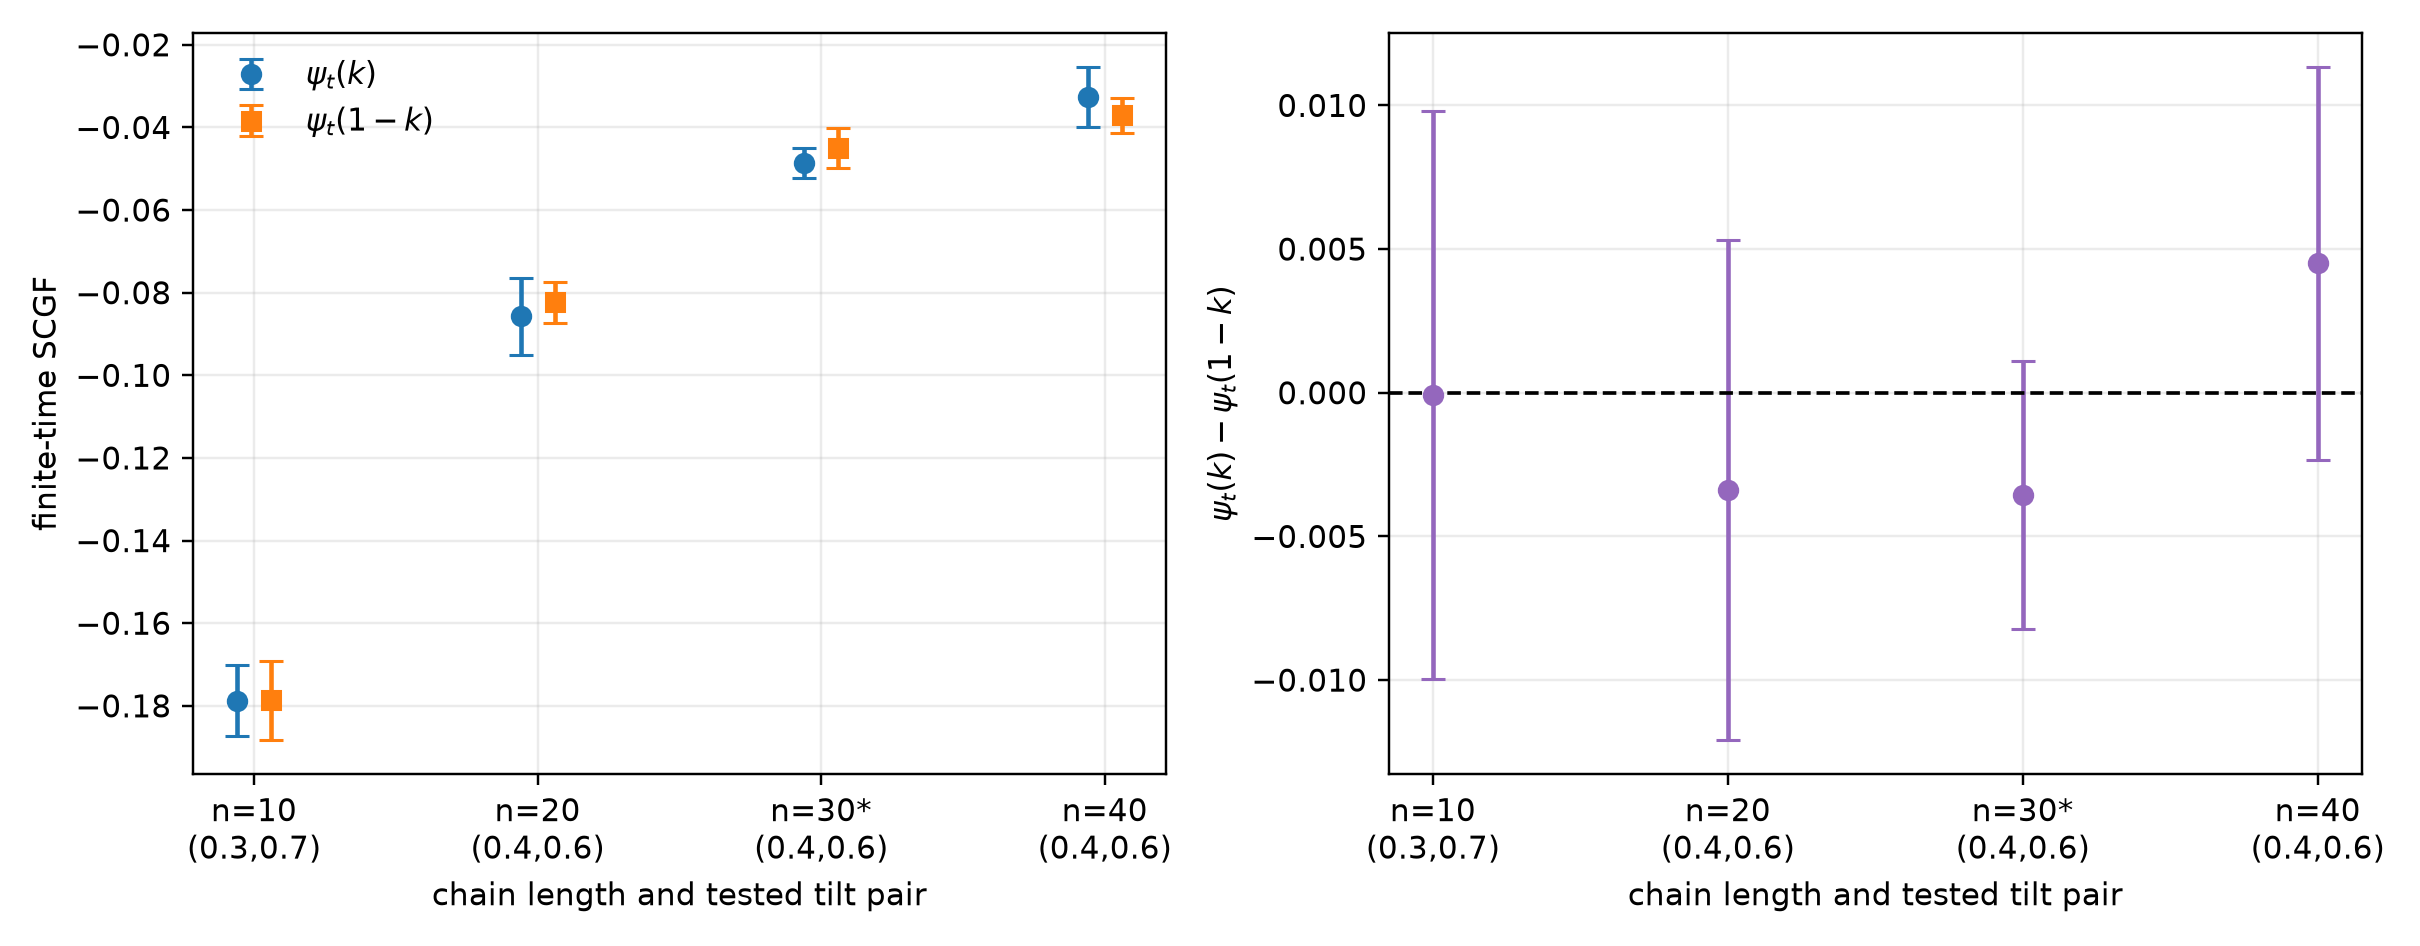
\includegraphics[width=\textwidth]{../final_summary/long_chain_gc_summary.png}
  \caption{Resolved paired SCGFs (left) and GC residuals (right).  Error bars
  are independent-run 95\% intervals.  The pair differs at $n=10$ and the
  longer chains because $(0.3,0.7)$ is not supported there.  The asterisk
  marks a row whose final population-convergence audit is unresolved.}
  \label{fig:gc-summary}
\end{figure}

For every row in Table~\ref{tab:gc}, the paired residual interval contains
zero and the support, late-half, and observation-time gates pass.  The
$n=30$ pair nevertheless remains unresolved because its individual $k=0.4$
SCGF changes by $-0.00347$ from $N_c=1024$ to $2048$, about $2.36$ combined
standard errors and hence beyond the frozen population-convergence gate.  The
paired residual can hide a common population bias through cancellation, so it
is not promoted to a positive result.  The separate timestep and
selection-interval results are reported below rather than folded into the same
error bars.

\section{Numerical sensitivity and failed diagnostics}

The endpoint chains were rerun after halving the timestep and after shortening
the selection interval from $2$ to $1$.  The supported final controls use
$N_c=1024$, $t=60$ at $n=10$ and $N_c=512$, $t=120$ at $n=40$.  The middle
lengths use the same integrator and estimator settings; the endpoint tests are
the least and most demanding members of the tested length range.  Earlier
unsupported lower-population or selection-4 controls are retained separately
as failed diagnostics.

\begin{table}[ht]
\centering
\small
\caption{Numerical controls relative to the frozen baseline.  The member
column is the larger absolute change among the two SCGF values; the next two
columns are changes in the full-window and late-half paired residuals.}
\label{tab:controls}
\begin{tabular}{rllrrrl}
\toprule
$n$ & control & pair & max. member $|\Delta\psi|$ & $\Delta D$ &
$\Delta D_{\rm late}$ & gate \\
\midrule
10 & selection interval & $(0.3,0.7)$ & 0.00242 & -0.00324 & -0.00405 & pass \\
10 & timestep halving & $(0.3,0.7)$ & 0.00455 & -0.00214 & -0.00104 & pass \\
40 & selection interval & $(0.4,0.6)$ & 0.00573 & +0.00747 & +0.01031 & fail \\
40 & timestep halving & $(0.4,0.6)$ & 0.00357 & +0.00198 & -0.00029 & pass \\
\bottomrule

\end{tabular}
\end{table}

Three of the four final endpoint-control rows pass.  At $n=40$, timestep
halving passes, but the supported selection-interval change $2\to1$ does not:
the $k=0.4$ member changes by $0.00573$ (about $2.84$ combined standard
errors), and the late-half paired residual changes by $0.01031$, just beyond
the unchanged absolute $0.01$ gate.  The earlier selection-4 series is also
retained as a failed diagnostic because its high-tilt member loses weight-ESS
support.  No further interval is selected from these results.

The first $n=40$, $N_c=1024$ production series at $t=60/80$ also remains a
failed diagnostic: its late-half residual exceeded $0.01$.  It was not pooled
with the independently seeded remedial $t=120$ series.

All rejected diagnostics remain part of the experiment record.  In
particular, the original all-chain target $(0.3,0.7)$ is not resolved for
$n\ge20$; no full-tilt-interval claim is made.  Early undercontrolled,
overcontrolled, and over-frequent-resampling pilots show low weight support or
genealogical collapse and are not counted as positive evidence.  The resulting
scope is therefore narrower than the original strongest target, but it is not
selected by deleting adverse runs.

\section{Conclusion}

The complete frozen estimator-and-control suite is numerically consistent with
the Gallavotti--Cohen SCGF symmetry over $(0.3,0.7)$ at $n=10$.  The core
paired-SCGF diagnostics are also consistent with the secondary pair
$(0.4,0.6)$ at $n=20$ and at the remedial $t=120$ horizon for $n=40$, but the
predeclared endpoint selection audit does not pass at $n=40$; hence these are
not promoted to a fully controlled all-long-chain claim.  At $n=30$, the
paired residual is consistent with zero but the individual population-
convergence audit fails.  The study therefore supplies a validated finite-chain
result at $n=10$ and transparent positive-but-incomplete long-chain evidence,
not a proof of the fluctuation theorem, not evidence over the unresolved
high-tilt interval, and not an infinite-chain statement.

\begin{thebibliography}{9}
\bibitem{LebowitzSpohn1999}
J.~L. Lebowitz and H. Spohn,
``A Gallavotti--Cohen-type symmetry in the large deviation functional for
stochastic dynamics,'' \emph{J. Stat. Phys.} 95, 333--365 (1999).
\bibitem{TailleurLecomte2009}
J. Tailleur and V. Lecomte,
``Simulation of large deviation functions using population dynamics,''
\emph{AIP Conf. Proc.} 1091, 212--219 (2009).
\bibitem{Nemoto2016}
T. Nemoto, E. Guevara Hidalgo, and V. Lecomte,
``Finite-time and finite-size scalings in the evaluation of large-deviation
functions: Analytical study using a birth-death process,''
\emph{Phys. Rev. E} 95, 012102 (2017).
\end{thebibliography}

\end{document}
